\chapter{Introduction}
\label{ch:introduction}

\def\figdir{chapters/introduction/figures/}

%\epigraph{\textit{The easiest way to solve a problem is to deny it exists.}}{Isaac Asimov}

%\begin{quote} 
%	\begin{flushright}
%		\textit{The easiest way to solve a problem\\ is to deny it exists.}
%		
%		--- ~ Prof. Isaac Asimov
%	\end{flushright}
%\end{quote}

\lettrine[lines=3,nindent=0em,loversize=0.1]{T}{he} global population is steady rising and migrating from rural areas to urban areas and results in a growing urbanization as urban for past two centuries. This result of a rapid rise in urban population and therefore in future the ecology of the urban system will become a primary concern. Furthermore, climate change, driven by human activity need to be reduces to mitigate the present detrimental climatology in urban areas. A lack thereof can not only have implication on the global climate but also the comfort and health of urban populace. 

Vegetation is agglomeration of leaves, needles, twigs and branches. Multiple and randomly oriented surfaces. First approximation, porous body. 

%The characteristics of the flow is also related to the pore size distribution. 

 Figure \ref{fig:vegetation_fluxes} shows a schematic representation of the various fluxes exchanged between an urban tree and the environment. 

\begin{figure}[h]
	\centering
	%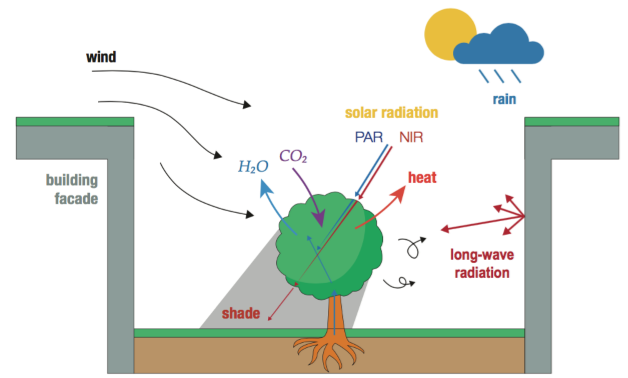
\includegraphics[width=0.7\textwidth]{\figdir/vegetation_fluxes.png}
	\caption{Interaction of urban vegetation with the urban microclimate.}
	\label{fig:vegetation_fluxes}
\end{figure}	

\section{Motivation}


\begin{itemize}
	\item Quantitative method to determine the amelioration of urban climate due to vegetation.
	\item Influence of vegetation on urban heat, mass and momentum exchanges in urban environment.
	\item Understand three-dimensional flow and radiation field change due to vegetation.
	\item Influence of vegetation on pedestrian thermal comfort. 
\end{itemize}

\section{Research questions}


\section{Scope and Methodology}

\section{Outline of the dissertation}

%\begin{spacing}{3.0}



%\blindmathpaper 

%\end{spacing}